\documentclass[12pt]{article}
\usepackage[utf8]{inputenc}
\usepackage[T2A]{fontenc}
\usepackage[russian]{babel}
\usepackage{amsmath}
\usepackage{amssymb}
\usepackage{dsfont}
\usepackage[dvipsnames]{xcolor}
\usepackage{setspace}
\usepackage{multirow}
\usepackage[a4paper, outer=1.5cm, inner=1.5cm, top=1cm, bottom=1cm]{geometry}
\usepackage{graphicx}
\usepackage{skull}
\usepackage{wasysym}
\usepackage{float}
\graphicspath{{.images/}}
\usepackage{hyperref}
\hypersetup{colorlinks=true, linkcolor=blue, filecolor=magenta, urlcolor=cyan}
\usepackage[firstpage]{draftwatermark}
\SetWatermarkText{
    $\qquad\qquad\qquad\qquad\qquad$\parbox{7cm}{\begin{center}
    
\includegraphics[width = 0.08\textwidth]{lion-logo.png}\bigskip\\~\bigskip\\~\vspace{-24mm}\\~\end{center}}
}
\SetWatermarkAngle{0}
\SetWatermarkScale{1.5}
\usepackage{etoolbox}

\newtoggle{ifsolved}
\newtoggle{needhelp}
\newcounter{num}
\setcounter{num}{1}

\newcommand{\newnum}{\par\textbf{\textnumero\arabic{num}}\stepcounter{num}}
\newcommand{\sol}{\vspace{3mm}\par\textbf{Решение: }}
\newcommand{\ans}{\vspace{3mm}\par\textbf{Ответ: }}
\newcommand{\hint}{\vspace{3mm}\par\textbf{Подсказка: }}
\newcommand{\mode}[1]{
\ifstrequal{#1}{0}{\togglefalse{ifsolved}\togglefalse{needhelp}}{\ifstrequal{#1}{1}{\togglefalse{ifsolved}\toggletrue{needhelp}}{\ifstrequal{#1}{2}{\toggletrue{ifsolved}\togglefalse{needhelp}}{\toggletrue{ifsolved}\toggletrue{needhelp}}}}} %if 0 - if 1 - if 2 - else
%\newenvironment{problem}[8]{%#1, #2, #3
%\parbox{\linewidth}{\vspace{4mm}\ifstrequal{#4}{(лёгкая)}{\newnum\textbf{.}}{\newnum\textbf{*.} } \\ #5}
%\iftoggle{ifsolved}{\sol #6}{}
%\iftoggle{ifsolved}{\ans #7}{}
%\iftoggle{needhelp}{\hint #8}{}}

\newenvironment{problem}[8]{%#1, #2, #3
\parbox{\linewidth}{\vspace{5mm}\ifstrequal{#4}{(лёгкая)}{\newnum\textbf{.}}{\newnum\textbf{*.} } \\ #5}
\iftoggle{ifsolved}{\sol #6}{}

\iftoggle{ifsolved}{\parbox{\linewidth}{\ans #7}}{}
\iftoggle{needhelp}{\parbox{\linewidth}{\hint #8}}{}}

\newenvironment{mylist} %custom list
{ \begin{itemize}
    \setlength{\itemsep}{0pt}
    \setlength{\parskip}{0pt}
    \setlength{\parsep}{0pt}     }
{ \end{itemize}                  }

\newenvironment{homeass}[1]{\vspace*{-1.5cm}
\iftoggle{ifsolved}{
    \section*{\center{Решение домашнего задания к #1.}}
}{
    \section*{\center{\textcolor{Sepia}{Домашнее задание к #1}}}
} \vspace{7mm}\large}

\parindent=0pt
\pagestyle{empty}
%$\!$[\arabic{class}.\arabic{num}]
%\ifnumcomp{\value{counter}}{>}{1}{true}{false}
%\definecolor{Gray}{gray}{0.9}
%\definecolor{mypink}{RGB}{219, 48, 122}
%\newcolumntype{g}{>{\columncolor{Gray}}p{2.8cm}}

\begin{document}
\large
\mode{7}
%0 for problems without hints
%1 for problems + hints
%2 for problems + solutions + answers
%else: show all

{\centering\section*{СПИСОК ЗАДАЧ}}

{\centering\subsection*{\smallskip\\\textcolor{green}{\textbf{Полезные вещи, которые можно и нужно копипастить:}}}}

\subsection*{\textcolor{Emerald}{\textbf{Полезные шпаргалки по LaTeXу:}}}

\textbf{Пример вставки рисунка:}

\begin{minipage}{\linewidth}
    \begin{minipage}{0.54\linewidth}
    см. рисунок справа\\
    Текст к собственно пикче, примерно всегда это либо развёрнутое описание, либо большая часть решения задачи --- стремимся экономить пространство, если это можно сделать.
    \end{minipage}
    \hspace{0.05\linewidth}
    \begin{minipage}{0.4\linewidth}
    \begin{figure}[H] 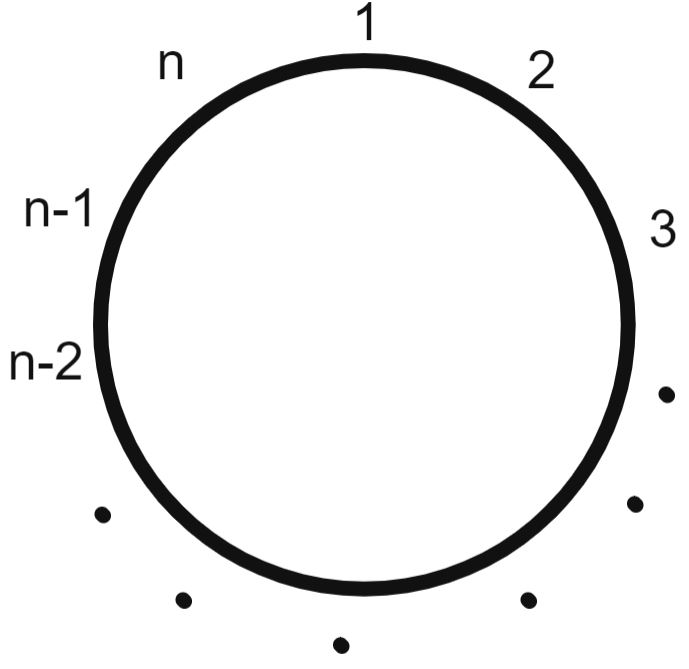
\includegraphics[width=\linewidth]{sol3} %тут поменять имя пикчи
    \end{figure}
    \end{minipage}
\end{minipage}

\textbf{Дефолтные математические знаки и символы:}\\
$\geqslant$,
$\leqslant$,
$a^{b}$,
$x_{i}$,
$\sqrt{a}$,
$\frac{a}{b}$,
$\displaystyle \frac{a}{b}$,
$\cdot$
$\;\Rightarrow\;$,
$\;\Leftrightarrow\;$,
$1{,}2$.
О промежутках:
$a\!b$,
$a\,b$,
$a\:b$,
$a\;b$,
$a\quad b$.

\textbf{Стандартные система и совокупность уравнений / неравенств:}\\
$\left\{
\begin{aligned}
f(x) &= 0 \\
g(x) &= 1
\end{aligned}\right.$

$\left[\begin{aligned}
&\left\{\begin{aligned}
f(x) &\geqslant a \\
g(x) &= b
\end{aligned}\right.\\
&\left\{\begin{aligned}
f(x) &< a \\
g(x) &= -b
\end{aligned}\right.
\end{aligned}\right.$

\subsection*{\textcolor{Emerald}{\textbf{Не математическое, но полезное:}}}
% комментарий в любом месте документа, который нигде не будет видно. Можно использовать для написания заметок-вопросов по задачам
\textbf{Пример таблицы:}

\begin{tabular}{|c|c|c|}
\hline
    $a$ & $b$ & текст
\\\hline
    $c$ & $d$ & мораль
\\\hline
\end{tabular}\\

\textbf{Отступы:} между\smallskip\\ строками\medskip\\ \textbf{Тире} --- это три дефиса.\\
\textbf{Списки:}
\begin{mylist}
\item [$\bullet$] это был пункт а
\item [2)] а это уже пункт номер 2 с изменённым заголовком
\end{mylist}

\subsection*{\textcolor{Emerald}{\textbf{Всё, неупомянутое выше (или если просто что-то не так):}}}
\begin{mylist}
\item [$\bullet$] Решение отдельных вопросов касательно ТеХа нужно искать в \href{https://www.mccme.ru/free-books/llang/newllang.pdf}{Львовском}.

\item [$\bullet$] Найти произвольный символ, который нужен, можно в \href{http://detexify.kirelabs.org/classify.html}{Detexify}.

\item [$\bullet$] Если возникли сомнения при решении, ответ практически ко всем задачам можно проверить с помощью \href{https://www.wolframalpha.com/}{WolframAlpha}.

\item [$\bullet$] Если в задаче нужно создать картинку, то лучше пока отложить эту задачу. Все графики планируется централизованно нарисовать (или перерисовать) в геогебре.

\item [\textcolor{brown}{\textbf{!!}}] Важно ставить \textcolor{red}{\textbf{$\spadesuit$}}
(или просто red) в тело задачи в случае серьёзных вопросов к решению и какой-то вопиющей лажи.

\item [\textcolor{brown}{\textbf{!!}}] Важно ставить \textcolor{olive}{\textbf{$\spadesuit$}}
(или просто olive) в тело задачи в случае не самого удачного текста и кривых отступов.
\end{mylist}

\subsection*{\textcolor{Violet}{\textbf{Комментарии:}}}% а также невидимые комментарии - так можно оставлять заметки-вопросы прямо в задаче, чтобы потом было понятно, в чём вопрос.
\begin{mylist}
\item [$\skull$] Переставлять задачи местами --- очень плохая идея.

\item [$\smiley$] При двойном клике по тексту pdf справа происходит автоматический переход к этому месту в латех-коде, а для обратного перехода можно нажать стрелку вправо (висит сверху между pdf и латех-кодом).

\item [$\smiley$] Если есть размышления, дописывать red/olive к задаче или не дописывать, то лучше всё-таки дописать.

\item [$\skull$] Самое плохое, что можно сделать --- написать в любое поле из трёх (НаписанноеРешение/ВерныйОтвет/Подсказка) только половину того, что надо, никак это не отметить, и потом пойти дальше.\\ Нужно в этот момент писать red/olive в случайном месте задачи, чтобы потом вычислить это с помощью Ctrl+F по всему документу (и это то, что потом будет делаться долго и тщательно)
\end{mylist}

\newpage
\setcounter{num}{528}

\hypertarget{7.2}{{\centering\section*{\bigskip\\\textcolor{Blue}{\hyperlink{start2}{\textcolor{Blue}{7.2}} Решение линейных систем.}\vspace{-5mm}}}}

\begin{problem}{Решение системы методом подстановки.}{7.2.2}{7A \textcolor{red}{\textbf{$\spadesuit$}}}{(лёгкая)}
{При каком значении параметра $b$ прямая $x + y = b$ пересекает прямую $5x - 3y = 16$ в точке, принадлежащей прямой $y + 2x = 0$?}
{НаписанноеРешение}
{ВерныйОтвет}{Подсказка}
\end{problem}

\begin{problem}{Решение системы методом подстановки.}{7.2.2}{7A \textcolor{red}{\textbf{$\spadesuit$}}}{(лёгкая)}
{При каком значении параметра $b$ прямая $x + y = b$ пересекает прямую $5x + 3y = 2$ в точке, принадлежащей прямой $y + 3x = 0$?}
{НаписанноеРешение}
{ВерныйОтвет}{Подсказка}
\end{problem}

\begin{problem}{Решение системы методом подстановки.}{7.2.2}{7A}{(лёгкая)}
{Решить систему уравнений: $\;\left\{
\begin{aligned}
    \: 3x + y &= 5\\
    \: \frac{x + 2}{5} &+ \frac{y}{2} = -1
\end{aligned}\right.$}
{НаписанноеРешение}
{ВерныйОтвет}{Подсказка}
\end{problem}

\begin{problem}{Решение системы методом подстановки.}{7.2.2}{7A \textcolor{red}{\textbf{$\spadesuit$}} мб сложновато}{*}
{Найти наименьшее значение выражения $|6x + 5y + 7| + |2x + 3y + 1|$ и значения $x$ и $y$, при которых оно достигается.}
{НаписанноеРешение}
{ВерныйОтвет}{Подсказка}
\end{problem}

\begin{problem}{Решение системы методом подстановки.}{7.2.2}{79I}{(лёгкая)}
{Даны три числа. Известно, что их сумма равна 120, первое составляет 60\% от суммы второго и третьего, а третье составляет 40\% от суммы первого и второго.\\ Найти эти числа.}
{НаписанноеРешение}
{ВерныйОтвет}{Подсказка}
\end{problem}

\begin{problem}{Решение системы методом подстановки.}{7.2.2}{6K \textcolor{olive}{\textbf{$\spadesuit$}}}{(лёгкая)}
{\vspace{-8mm}\\\begin{minipage}{\linewidth}
    \begin{minipage}{0.74\linewidth}
    ~\vspace{2mm}\\
    В квадрат вписали целые числа так, что их суммы в каждой строке, столбце и диагонали одинаковы.\\ Затем все числа, кроме трёх, стерли.\\
    Какое число было написано в клетке, отмеченной крестом?
    \end{minipage}
    \hspace{0.04\linewidth}
    \begin{minipage}{0.2\linewidth}
        \begin{figure}[H]
        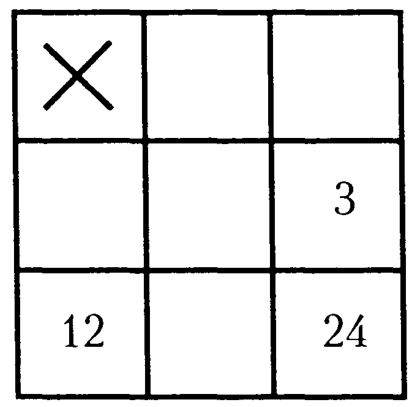
\includegraphics[width=\linewidth]{6K-19}
        \end{figure}
    \end{minipage}
\end{minipage}}
{Пусть в нижней клетке между 12 и 24 было написано некоторое неизвестное нам число $x$. Тогда сумма чисел в этой строке равна $12 + x + 24 = 36 + x$.\\
Тогда, поскольку все суммы должны быть одинаковы, несложно подметить, что в правом столбце сумма пока что равна $3 + 24 = 27$, а значит, в правом верхнем углу было написано число $x + 9$ (поскольку $27 + x + 9 = 36 + x$, см. рисунок слева)
\vspace{-8mm}\\\begin{minipage}{\linewidth}
    \begin{minipage}{0.2\linewidth}
        \begin{figure}[H]
        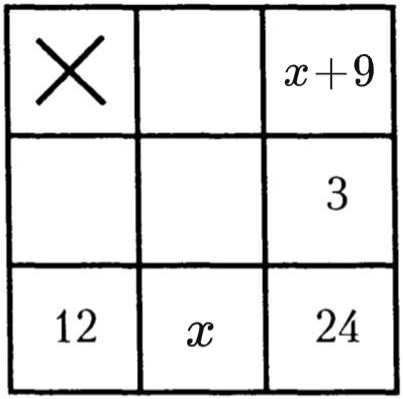
\includegraphics[width=\linewidth]{sol70}
        \end{figure}
    \end{minipage}
    \hspace{0.03\linewidth}
    \begin{minipage}{0.49\linewidth}
    ~\vspace{2mm}\\
    Можно заметить, что стоящие на диагонали числа $12$ и $x+9$ в сумме дают $21 + x$. А значит, поскольку сумма трёх чисел на диагонали равна $36 + x$, то в центральной клетке стоит число $15$. А в клетке выше --- 21 ($21 + 15 + x = 36 + x$).
    \end{minipage}
    \hspace{0.05\linewidth}
    \begin{minipage}{0.2\linewidth}
        \begin{figure}[H]
        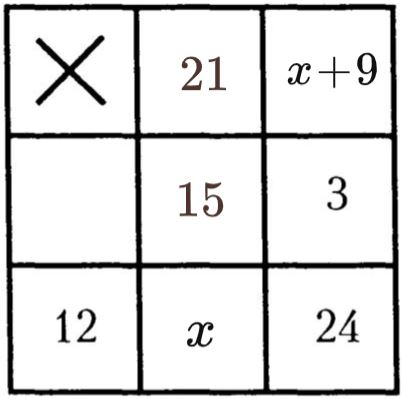
\includegraphics[width=\linewidth]{sol71}
        \end{figure}
    \end{minipage}
\end{minipage}
\smallskip\\
Теперь осталось отметить, что сумма двух чисел в верхней строке равна $30 + x$. А значит, число в левом верхнем углу --- 6.}
{В клетке, отмеченной крестом, было написано число 6.\\
\textbf{Комментарий:} Поскольку на диагонали стоят числа 6, 15, 24, сумма чисел равна $6+15+24 = 45$, и поэтому $x = 9$. Так можно найти все оставшиеся числа в таблице.}{Пусть в нижней клетке написано число $x$. Какое число тогда было написано в правом верхнем углу? А что за число было в центре?}
\end{problem}

\begin{problem}{Решение системы методом подстановки.}{7.2.2}{79I}{(лёгкая)}
{На опушке сосен вдвое больше, чем осин, тополей вдвое меньше чем берёз, сосен и берёз поровну, а число тополей составляет 75\% от числа сосен.\\ Кроме того, на опушке растёт один большой дуб, под которым лежит Андрей.\\ Могло ли такое быть?}
{НаписанноеРешение}
{ВерныйОтвет}{Подсказка}
\end{problem}

\begin{problem}{Решение системы методом подстановки.}{7.2.2}{6K red в примеры задач}{(лёгкая)}
{На лужайке росли $35$ жёлтых и белых одуванчиков.\\ После того, как $8$ белых облетели, а $2$ жёлтых побелели, жёлтых одуванчиков стало вдвое больше, чем белых.\\ Сколько белых одуванчиков росло на лужайке сначала? А жёлтых?}
{Как обычно, вводим неизвестные: пусть сначала жёлтых одуванчиков было $y$, а белых одуванчиков было $w$.\\ Мы знаем, что сначала было всего 35 одуванчиков, то есть $y + w = 35$.\\
Теперь второе условие. Когда 8 белых одуванчиков облетели, они перестали быть и белыми, и жёлтыми. То есть вместо 35 одуванчиков теперь белых и жёлтых только $35 - 8 = 27$. Так как двое жёлтых побелели, жёлтых теперь на два меньше (то есть $y - 2$), а белых на 2 больше (то есть $w + 2$).\smallskip\\ Главное~--- не забыть, что 8 белых всё же облетели, и на самом деле белых уже $w + 2 - 8 = w - 6$.\smallskip\\
Итого: в конце у нас $y - 2$ жёлтых и $w - 6$ белых. Мы знаем, что всего их 27 и что жёлтых стало вдвое больше, чем белых. То есть задача~--- разделить 27 в отношении $1:2$. Получаем 9 и 18 (9 белых, 18 жёлтых).\\
$9 = w - 6 \;\Rightarrow\; w = 15$\hfill
$18 = y - 2 \;\Rightarrow\; y = 20$.\smallskip\\
Делаем проверку:\\ 20 жёлтых, 15 белых $\:\xrightarrow{\text{8 облетели}}\:$ 20 жёлтых, 7 белых $\:\xrightarrow{\text{2 побелели}}\:$ 18 жёлтых, 9 белых.

}
{Сначала было 20 жёлтых и 15 белых одуванчиков.}{Подсказка}
\end{problem}

\begin{problem}{Решение системы методом подстановки.}{7.2.2}{9I}{(лёгкая)}
{В сосуд, содержащий 7 литров 15-процентного водного раствора некоторого вещества (медного купороса $\text{Cu}_2 \text{SO}_4$), добавили 8 литров воды.\\ Сколько процентов составит концентрация получившегося раствора?}
{НаписанноеРешение}
{ВерныйОтвет}{Подсказка}
\end{problem}

\begin{problem}{Решение системы методом подстановки.}{7.2.2}{6S}{(лёгкая)}
{Разность двух чисел равна $44\frac{1}{2}$. Если меньшее из них увеличить в 7 раз, то новая разность будет равна $10\frac{3}{14}$. Найти эти числа.}
{НаписанноеРешение}
{ВерныйОтвет}{Подсказка}
\end{problem}

\begin{problem}{Решение системы с помощью алгебраических преобразований.}{7.2.3}{6S}{(лёгкая)}
{Сумма двух чисел равна $11\frac{1}{5}$, а разность их равна 9. Найти эти числа.}
{НаписанноеРешение}
{ВерныйОтвет}{Подсказка}
\end{problem}

\begin{problem}{Решение системы с помощью алгебраических преобразований.}{7.2.3}{7A \textcolor{red}{\textbf{$\spadesuit$}} не было модуля}{(лёгкая)}
{Решить уравнение: $|x + y + 3| + |y + z + 4| + |x + z + 5| = 0$.}
{НаписанноеРешение}
{ВерныйОтвет}{Подсказка}
\end{problem}

\begin{problem}{Решение системы с помощью алгебраических преобразований.}{7.2.3}{7A}{(лёгкая)}
{Сумма цифр двузначного числа равна 12. Если эти цифры поменять местами, то получится число, которое на 36 меньше исходного. Найти эти числа.}
{НаписанноеРешение}
{ВерныйОтвет}{Подсказка}
\end{problem}

\begin{problem}{Решение системы с помощью алгебраических преобразований.}{7.2.3}{79I}{(лёгкая)}
{На олимпиаду по географии от каждой школы отправили двух или трёх учащихся. Всего в олимпиаде участвовало 65 учащихся из 24 разных школ.\\ Сколько школ отправили на олимпиаду трёх учащихся?}
{НаписанноеРешение}
{ВерныйОтвет}{Подсказка}
\end{problem}

\begin{problem}{Решение системы с помощью алгебраических преобразований.}{7.2.3}{6S}{(лёгкая)}
{\begin{minipage}{\linewidth}
    \begin{minipage}{0.12\linewidth}
        \begin{figure}[H]
        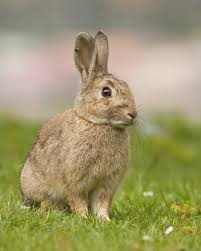
\includegraphics[width=\linewidth]{6K-48}
        \end{figure}
    \end{minipage}
    \hspace{0.03\linewidth}
    \begin{minipage}{0.58\linewidth}
    ~\vspace{1mm}\\
    В клетке находятся фазаны и кролики.\\ Известно, что у них вместе 35 голов и 94 ноги.\\ Сколько в клетке фазанов и сколько кроликов?
    \end{minipage}
    \hspace{0.03\linewidth}
    \begin{minipage}{0.2\linewidth}
        \begin{figure}[H]
        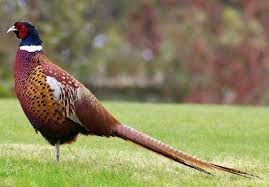
\includegraphics[width=\linewidth]{6K-49}
        \end{figure}
    \end{minipage}
\end{minipage}}
{Пусть всего было $p$ фазанов и $r$ кроликов.\\ Тогда $p + r = 35$ (количество голов~--- это число кроликов и фазанов вместе) и $2p + 4r = 94$ (у каждого фазана две ноги, у каждого кролика 4 ноги).\\ Значит, $\left\{\begin{aligned}
p + r\;\, &= 35\\
2p + 4r &= 94
\end{aligned}\right.\quad$ Домножим первое уравнение на 2 и вычтем его из второго уравнения: получаем, что $2p + 4r - 2p - 2r = 94 - 35\cdot 2 \;\Rightarrow\; 2r = 24 \;\Rightarrow$\\$\Rightarrow r = 12 \;\Rightarrow\; p = 35 - 12 = 23$. Итого, всего в клетке 23 фазана и 12 кроликов.}
{В клетке было 23 фазана и 12 кроликов.}{Можно умножить первое уравнение на 2 (или поделить второе уравнение на 2), а затем вычесть.}
\end{problem}

\begin{problem}{Решение системы с помощью алгебраических преобразований.}{7.2.3}{6S}{(лёгкая)}
{В хозяйстве есть куры и овцы.\\ Сколько тех и других, если известно, что вместе у них всех 19 голов и 46 ног?}
{НаписанноеРешение}
{ВерныйОтвет}{Подсказка}
\end{problem}

\begin{problem}{Решение системы с помощью алгебраических преобразований.}{7.2.3}{6S}{(лёгкая)}
{В комнате стоят стулья и табуретки. У каждой табуретки 3 ноги, у каждого стула 4 ноги. Когда на всех табуретках и стульях сидят люди, в комнате всего 39 ног. Сколько стульев и табуреток в комнате?}
{НаписанноеРешение}
{ВерныйОтвет}{Подсказка}
\end{problem}

\begin{problem}{Решение системы с помощью алгебраических преобразований.}{7.2.3}{6K}{(лёгкая)}
{Масса семи одинаковых гаек и четырёх одинаковых болтов равна $115$ г, а масса таких же трёх гаек и четырёх болтов~--- $95$ г. Найти массу одного болта.}
{Пусть $\text{Г}$~--- масса одной гайки, а $\text{Б}$~--- масса одного болта (в граммах). Тогда, согласно первому условию, $7\text{Г} + 4\text{Б} = 115$г. Согласно же второму условию $3\text{Г} + 4\text{Б} = 95$г. Несложно заметить, что $4\text{Б} = 115 - 7\text{Г}$ и что $4\text{Б} = 95 - 3\text{Г}$, а это значит, что $115 - 7\text{Г} = 95 - 3\text{Г} \;\Rightarrow\; 115 - 95 = 7\text{Г} - 3\text{Г} \;\Rightarrow\; 20 = 4\text{Г} \;\Rightarrow\; \text{Г} = 5$г. То есть одна гайка весит 5 грамм. Находим, сколько весит болт: $4\text{Б} = 95 - 3\text{Г} = 95 - 3\cdot5 = 80 \;\Rightarrow\; \text{Б} = 20$г. Итого, один болт весит двадцать грамм.}
{Масса одного болта составляет 20 грамм.}{Пусть $\text{Г}$~--- масса одной гайки, а $\text{Б}$~--- масса одного болта...}
\end{problem}

\begin{problem}{Решение системы с помощью алгебраических преобразований.}{7.2.3}{6S}{(лёгкая)}
{За 6 карандашей, 4 ручки и блокнот заплатили 270 р. Один карандаш, одна ручка и блокнот стоят вместе столько же, сколько 3 карандаша и 3 ручки вместе, а именно 120 р. Сколько стоит каждая вещь отдельно?}
{НаписанноеРешение}
{ВерныйОтвет}{Подсказка}
\end{problem}

\begin{problem}{Решение системы с помощью алгебраических преобразований.}{7.2.3}{6S}{(лёгкая)}
{Пакет, в котором 3 яблока и 8 мандаринов, весит 620 г, а пакет, в котором 3 яблока и 5 мандаринов, весит 500 г. Какова масса 1 яблока и 1 мандарина?}
{НаписанноеРешение}
{ВерныйОтвет}{Подсказка}
\end{problem}

\begin{problem}{Решение системы с помощью алгебраических преобразований.}{7.2.3}{6K}{(лёгкая)}
{Первая дама купила в магазине 3 больших попугая и двух маленьких, а вторая дама купила одного большого попугая и четырех маленьких попугайчиков.\\ Сколько стоят большие попугаи и сколько~--- маленькие, если первая дама заплатила 15000 рублей, а вторая~--- 10000 рублей?}
{НаписанноеРешение}
{ВерныйОтвет}{Подсказка}
\end{problem}

\begin{problem}{Решение системы с помощью алгебраических преобразований.}{7.2.3}{6S}{(лёгкая)}
{5 помидоров и 2 огурца весят столько же, сколько 9 помидоров и 1 огурец.\\ Что тяжелее: 8 помидоров или 2 огурца?}
{Пусть $t$~--- вес одного помидора, а $c$~--- вес одного огурца.\\ Имеем $5t + 2c = 9t + c \;\Rightarrow\;c = 4t$. То есть огурец весит столько же, сколько и 4 помидора. Тогда очевидно, что два огурца весят столько же, сколько 8 помидоров, и следовательно ответ~--- они весят одинаково.}
{8 помидоров весят столько же, сколько и 2 огурца.}{Ввести две неизвестные и решить получившееся уравнение.}
\end{problem}

\begin{problem}{Решение системы с помощью алгебраических преобразований.}{7.2.3}{6S}{(лёгкая)}
{3 утёнка и 4 гусёнка весят 2 кг 500 г, а 4 утёнка и 3 гусёнка весят 2 кг 400 г. Сколько весит 1 гусёнок?}
{НаписанноеРешение}
{ВерныйОтвет}{Подсказка}
\end{problem}

\begin{problem}{Решение системы с помощью алгебраических преобразований.}{7.2.3}{6K \textcolor{olive}{\textbf{$\spadesuit$}}}{(лёгкая)}
{\vspace{-6mm}\\\begin{minipage}{\linewidth}
    \begin{minipage}{0.5\linewidth}

    Новогодний подарок упакован в коробку с квадратным основанием. Высота коробки вдвое меньше стороны этого квадрата. Ленточкой длины $156$ см можно перевязать коробку и сделать бантик сверху (как на рисунке). А чтобы перевязать её с точно таким же бантиком сбоку (справа), нужна ленточка длины $178$ см. Найти размеры коробки.

    \end{minipage}
    \hspace{0.05\linewidth}
    \begin{minipage}{0.44\linewidth}
        \begin{figure}[H]
        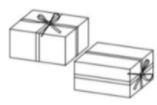
\includegraphics[width=\linewidth]{6K-14}
        \end{figure}
    \end{minipage}
\end{minipage}}
{НаписанноеРешение}
{ВерныйОтвет}{Подсказка}
\end{problem}

\begin{problem}{Решение системы с помощью алгебраических преобразований.}{7.2.3}{6K}{(лёгкая)}
{А и Б собрали $21$ гриб, Б и В собрали $33$ гриба, а А и В собрали $24$ гриба.\\ Сколько собрал каждый?}
{НаписанноеРешение}
{ВерныйОтвет}{Подсказка}
\end{problem}

\begin{problem}{Решение системы с помощью алгебраических преобразований.}{7.2.3}{6K}{*}
{Первая и вторая труба наполняют бассейн за $9$ часов, вторая и третья~--- за $18$ часов, а первая и третья~--- за $12$ часов.\\ За сколько минут наполнят бассейн эти три трубы, работая одновременно?}
{НаписанноеРешение}
{ВерныйОтвет}{Подсказка}
\end{problem}

\begin{problem}{Решение системы с помощью алгебраических преобразований.}{7.2.3}{6S}{(лёгкая)}
{Найти ошибку в рассуждении:\\
$\begin{aligned}
    x &= \frac{1}{3};\\
    3x &= 1;\\
    15x - 12x &= 5 - 4;\\
    15x - 5 &= 12x - 4;\\
    5 \cdot (3x - 1) &= 4 \cdot (3x - 1);\\
    5 &= 4.
\end{aligned}$}
{НаписанноеРешение}
{ВерныйОтвет}{Подсказка}
\end{problem}

\begin{problem}{Решение системы с помощью алгебраических преобразований.}{7.2.3}{79I}{(лёгкая)}
{Решить систему уравнений $\quad\left\{
\begin{aligned}
    \: 3x + 4y - 10 &= 0\\
    \: 5y - 4x + 3 &= 0
\end{aligned}\right.$}
{НаписанноеРешение}
{ВерныйОтвет}{Подсказка}
\end{problem}

\begin{problem}{Решение системы с помощью алгебраических преобразований.}{7.2.3}{6S}{(лёгкая)}
{Самое большое из трёх неизвестных чисел больше самого малого на $2{,}4$.\\ Если одно из них умножить на 12, другое~--- на 15, а третье на 10, полученные произведения окажутся равными. Найти эти числа.}
{НаписанноеРешение}
{ВерныйОтвет}{Подсказка}
\end{problem}

\begin{problem}{Решение системы с помощью алгебраических преобразований.}{7.2.3}{7A}{*}
{Велосипедист и пешеход вышли из А в В. Когда велосипедист доезжает до пункта В, он разворачивается и едет в А, потом опять разворачивается, и так далее. Пешеход же движется по прямой. Скорости и у пешехода, и у велосипедиста постоянны, и известно, что время с момента выхода до первой их встречи равно 35 минутам. Сколько времени пройдёт после этого до их пятой встречи?\\ (Известно, что пешеход к этому моменту ещё не дойдёт до пункта В)}
{Чтобы разобраться с этой каверзной задачей, надо сначала понять, в чём именно вопрос, а значит, понять, что такое первая и пятая встреча велосипедиста и пешехода. С первой встречей понятно: пешеход прошёл некоторое расстояние, а велосипедист доехал до В, развернулся, и доехал до пешехода.\smallskip\\ Понятное дело, мы не знаем точно место, где произошла встреча, но кое-что нам всё же известно: мы знаем, что вместе пешеход и велосипедист за это время \textbf{два} раза прошли расстояние от А до В. Что насчёт пятой встречи? Пешеход продолжает двигаться по прямой, а для велосипедиста же картина следующая: он доехал до В --- встретил пешехода (1 встреча) --- доехал до А --- догнал пешехода (2 встреча) --- доехал до В --- встретил пешехода снова (3 встреча) --- доехал до А --- догнал пешехода снова (4 встреча) --- доехал до В --- 5 встреча.\smallskip\\
То есть велосипедист 5 раз проехал расстояние между А и В, а потом проехал ещё некоторую часть и встретил пешехода. Это значит, что к этому моменту времени велосипедист и пешеход суммарно \textbf{шесть} раз прошли расстояние от А до В.\smallskip\\
После непродолжительных раздумий, становится ясно, что так как оба двигаются туда-сюда без остановок, с начала движения до пятой встречи пройдёт втрое больше времени, чем с начала движения до первой встречи (там они прошли расстояние два раза, а к пятой встрече --- уже шесть раз).\\ Значит, с начала движения до 5 встречи пройдёт $35 \cdot 3 = 105$ минут. Поэтому время между 1 и 5 встречей составляет $105 - 35 = 70$ минут, или 1 час 10 минут.}
{С первой встречи до пятой пройдёт 1 час 10 минут, или 70 минут.}{Сколько расстояний от А до В они пройдут вместе с начала движения до первой встречи? А сколько будет этих расстояний в момент пятой встречи?\\
Перед тем, как давать ответ, проверь, что найдено время \textbf{между} 1 и 5 встречей.}
\end{problem}

\begin{problem}{Решение системы с помощью алгебраических преобразований.}{7.2.3}{6K}{*}
{Двое идут по прямой дороге $AB$. Один идёт пешком из $A$ в $B$, другой стартует из $B$ в то же время, что и первый, и в отличие от него, второй быстро бегает туда-обратно без остановок.
\\a) Известно, что время с начала движения до их первой встречи равно $6$ минутам. Сколько времени пройдёт с начала движения до их третьей встречи, если к этому моменту пешеход всё ещё не дошёл до $B$?
\\b) Известно, что расстояние между точками $A$ и $B$ равно $2$ км, а скорость пешехода в $3$ раза меньше скорости бегуна.\\ Нарисовать график, показывающий расстояние до $B$ для обоих человек (нарисовать разными цветами для первого и второго).\\ Через сколько минут после третьей встречи пешеход прибудет в $B$? А бегун?}
{НаписанноеРешение}
{ВерныйОтвет}{Подсказка}
\end{problem}

\begin{problem}{Решение системы с помощью алгебраических преобразований.}{7.2.3}{9D}{*}
{Найти $9x + 11y - 6z + 7t + 5m$, если
$\;\left\{\begin{aligned}
    2x + 3y - z + t + m &= 4\\
    -x + y + 2z - 3t - m &= -3
\end{aligned}\right.$}
{Единственный шанс найти эту комбинацию с пятью различными буквами --- если мы сможем её соорудить из двух известных нам уравнений. То есть, если $P\cdot(2x + 3y - z + t + m) + Q\cdot(-x + y + 2z - 3t - m) = 9x + 11y - 6z + 7t + 5m$.\\
Как это получится? Мы должны получить девять иксов, 11 игреков, и так далее. А значит,
$\left\{\begin{aligned}
P\cdot2 &+ Q\cdot(-1) = 9 \;(\text{подсчёт } x)\\
P\cdot3 &+ Q\cdot1 = 11 \;(\text{подсчёт } y)\\
P\cdot(-1) &+ Q\cdot2 = -6 \;(\text{подсчёт } z)\\
P\cdot1 &+ Q\cdot(-3) = 7 \;(\text{подсчёт } t)\\
P\cdot1 &+ Q\cdot(-1) = 5 \;(\text{подсчёт } m).
\end{aligned}\right.$ \parbox{7cm}{После продолжительных размышлений, можно найти ответ:\\ $\vphantom{t}$~$\quad\quad P = 4$, $\quad Q = -1$.\\
Проверим, что все пять равенств выполняются:}
$\left\{\begin{aligned}
4\cdot2 + (-1)\cdot(-1) &= 9\\
4\cdot3 + (-1)\cdot1 &= 11\\
4\cdot(-1) + (-1)\cdot2 &= -6\\
4\cdot1 + (-1)\cdot(-3) &= 7\\
4\cdot1 + (-1)\cdot(-1) &= 5.
\end{aligned}\right.\quad\;$ \parbox{11cm}{Таким образом, $9x + 11y - 6z + 7t + 5m =\\= 4\cdot(2x + 3y - z + t + m) - 1\cdot(-x + y + 2z - 3t - m) = 4\cdot4 - 1\cdot(-3) = 16+3 = 19$.}}
{$9x + 11y - 6z + 7t + 5m = 19$.\\
\textbf{Комментарий:} Разумеется, тот факт, что верны одновременно 5 не связанных друг с другом уравнений --- большая удача.\\ В большинстве случаев такая хитрость, как в этой задаче, не сработает.}{Получить искомое выражение нужно из двух уже имеющихся!}
\end{problem}

\begin{problem}{Примеры из реальной жизни.}{7.2.4}{9I}{(лёгкая)}
{В абрикосах содержится 91\% влаги, а в кураге 7\% влаги.\\ Сколько граммов кураги получится из $21{,}7$ кг абрикосов?}
{НаписанноеРешение}
{ВерныйОтвет}{Подсказка}
\end{problem}

\begin{problem}{Примеры из реальной жизни.}{7.2.4}{9I \textcolor{red}{\textbf{$\spadesuit$}} матеммодель}{(лёгкая)}
{На уроке литературы учитель решил узнать, кто из 40 учеников класса летом читал книги <<Война и мир>> и <<Преступление и наказание>>.\\ Результаты опроса оказались таковы: <<Войну и мир>> читали 25 учащихся,\\ <<Преступление и наказание>>~--- 22 учащихся, обе книги читали 10 человек.\\ Сколько человек летом не прочитали ни одной из этих книг?}
{НаписанноеРешение}
{ВерныйОтвет}{Подсказка}
\end{problem}

\begin{problem}{Примеры из реальной жизни.}{7.2.4}{9I}{(лёгкая)}
{Ширина аквариума (прямоугольного параллелепипеда) составляет 80\% длины, а высота~--- 124\% длины.\\ Найти объём этого аквариума, если сумма длин рёбер его каркаса равна $60{,}8$ дм.

}
{НаписанноеРешение}
{ВерныйОтвет}{Подсказка}
\end{problem}

\begin{problem}{Примеры из реальной жизни.}{7.2.4}{6K}{(лёгкая)}
{Даша и Маша пропалывают грядку за 12 минут, а Маша в одиночку~--- за 20 минут. За сколько минут пропалывает грядку Даша, работая в одиночку?}
{НаписанноеРешение}
{ВерныйОтвет}{Подсказка}
\end{problem}

\begin{problem}{Примеры из реальной жизни.}{7.2.4}{9I}{(лёгкая)}
{Численность бобров в двух заповедниках в 2020 году составляла 220 особей.\\ Через год обнаружилось, что в первом заповеднике численность бобров увеличилась на 10\%, а во втором~--- на 20\%. В результате общая численность бобров в двух заповедниках составила 250 особей.\\ Сколько бобров было в первом заповеднике в 2020 году?}
{Для решения задачи сперва введём неизвестные. Пусть в 2020 году в первом заповеднике было $x$ бобров, а во втором заповеднике --- $y$ бобров.\\ Тогда после увеличения в первом заповеднике будет $1{,}1x$, а во втором $1{,}2y$.\\ Отсюда получаем два уравнения:
$\;\left\{\begin{aligned}
x &+ y = 220\\
1{,}1x &+ 1{,}2y = 250.
\end{aligned}\right.\quad$ Решаем систему.\\
$\left\{\begin{aligned}
x &+ y = 220\\
1{,}1x &+ 1{,}2y = 250
\end{aligned}\right. \;\Leftrightarrow\;
\left\{\begin{aligned}
1{,}1x &+ 1{,}1y = 242\\
1{,}1x &+ 1{,}2y = 250
\end{aligned}\right. \;\Leftrightarrow\;
\left\{\begin{aligned}
0{,}1y = 8\quad\;\\
x = 220 - y
\end{aligned}\right. \;\Leftrightarrow\;
\left\{\begin{aligned}
y &= 80\\
x &= 140.
\end{aligned}\right.$}
{В 2020 году в первом заповеднике было $140$ бобров (а во втором --- 80).}{Введи неизвестные: пусть в 2020 году в первом заповеднике было $x$ бобров, а во втором заповеднике --- $y$ бобров. Реши получившуюся систему.}
\end{problem}

\begin{problem}{Примеры из реальной жизни.}{7.2.4}{6S}{(лёгкая)}
{Для похода, совершаемого 46 школьниками, были приготовлены шестиместные и четырёхместные лодки. Сколько было тех и других лодок, если все туристы разместились в 10 лодках и свободных мест не осталось?}
{НаписанноеРешение}
{ВерныйОтвет}{Подсказка}
\end{problem}

\begin{problem}{Примеры из реальной жизни.}{7.2.4}{6S}{(лёгкая)}
{Вот крокодил и чемодан, их вес~--- две бочки и диван.\\
Чемодан без крокодила весит две корзины ила.\\
Ровно шесть корзинок ила весит чёрная горилла.\\
Две гориллы, посмотри, сколько бочек весят? Три.\\
И всё та же обезьяна весит ровно полдивана.\\
Сколько весит крокодил в пересчёте на горилл?}
{НаписанноеРешение}
{ВерныйОтвет}{Подсказка}
\end{problem}

\begin{problem}{Примеры из реальной жизни.}{7.2.4}{6S}{(лёгкая)}
{Акробат и собачонка весят два пустых бочонка.\\
Шустрый пёс без акробата весит два мотка шпагата.\\
А с одним мотком ягнёнок весит, видите, бочонок.\\
Сколько весит акробат в пересчёте на ягнят?}
{НаписанноеРешение}
{ВерныйОтвет}{Подсказка}
\end{problem}

\begin{problem}{Примеры из реальной жизни.}{7.2.4}{9D}{*}
{В набор <<Всё для школы>> входит 5 ручек разных цветов, карандаш, ластик, точилка, текстовый выделитель и линейка. В наборе же <<1 сентября>> меньше предметов: есть только 3 ручки, 2 текстовых выделителя, 2 карандаша и точилка. Также есть набор для черчения, в который входит 4 карандаша, точилка, два ластика и одна линейка. Можно ли, комбинируя эти наборы, купить ровно 19 ручек, 12 карандашей, 4 ластика, 6 точилок, 8 текстовых выделителей и 3 линейки? \\Сколько это всё вместе будет стоить, если известно, что набор <<Всё для школы>> стоит 289р, набор <<1~сентября>> стоит 226р, а набор для черчения стоит 244р?}
{Перепишем условие, чтобы было проще понять, что входит в набор:\smallskip\\
\textbf{№1} <<Всё для школы>>: 5 р. --- 1 кар. --- 1 ласт. --- 1 точ. --- 1 выд. --- 1 лин. --- 289руб.\\
\textbf{№2} $\;\;$ <<1~сентября>>: $\quad$ 3 р. --- 2 кар. --- 0 ласт. --- 1 точ. --- 2 выд. --- 0 лин. --- 226руб.\\
\textbf{№3} <<Для черчения>>: $\:$ 0 р. --- 4 кар. --- 2 ласт. --- 1 точ. --- 0 выд. --- 1 лин. --- 244руб.\\
$\vphantom{t}\;$ \textbf{Хотим купить:} $\;\,$ 19 р. --- 12 кар. --- 4 ласт. --- 6 точ. --- 8 выд. --- 3 лин. --- $x$ руб.\smallskip\\
Прийти к верному ответу можно несколькими способами, я приведу два:\smallskip\\
\textit{Путь решения №1}: Третий набор на количество ручек никак не влияет. Значит, нужно набрать 19 ручек с помощью первых двух наборов. Нельзя купить 4 первых набора --- тогда ручек будет слишком много. Нельзя купить три --- поскольку тогда никак не получится добрать ровно 4 ручки. По той же причине нельзя купить ни одного или 1 такой набор (19 и 14 не делятся на 3). Значит, первых наборов могло быть куплено только 2 (а вторых наборов в таком случае 3, и $2\cdot5 + 3\cdot3 = 19$). Исходя из количества карандашей понятно, что надо добавить ещё один третий набор. Далее проверка.\smallskip\\
\textit{Путь решения №2}: Количество карандашей должно быть чётно, а значит первых наборов должно быть чётное количество. Первых наборов не может быть 4 штуки или больше (тогда будет куплено 4 или более линеек), поэтому остаётся два варианта --- ни одного такого набора или 2. Но если не купить ни одного такого набора, то все ластики и линейки мы сможем получить только из третьего набора, и тогда ластиков будет в два раза больше, чем линеек. Противоречие.\\ Значит, таких наборов 2, для правильного количества ластиков и линеек надо добавить ещё один третий набор, а также три набора №2. Далее проверка.\smallskip\\
Проверка: в двух наборах <<Всё для школы>>, трёх наборах <<1~сентября>>, и наборе для черчения всего вместе $2\cdot5 + 3\cdot3 + 1\cdot0 = 19$ ручек, $2\cdot1 + 3\cdot2 + 1\cdot4 = 12$ карандашей, $2\cdot1 + 3\cdot0 + 1\cdot2 = 4$ ластика, $2 + 3 + 1 = 6$ точилок, $2\cdot1 + 3\cdot2 = 8$ текстовых выделителей, и $2\cdot1 + 3\cdot0 + 1\cdot1 = 3$ линейки. Всё совпадает.\\
Общая стоимость покупки в этом случае составит $2\cdot289 + 3\cdot226 + 1\cdot244 = 2\cdot(289 + 226) + (226 + 244) = 2\cdot515 + 470 = 1030 + 570 = 1600$ рублей.}
{Да, можно: надо купить два набора <<Всё для школы>>, три набора <<1~сентября>>, и один набор для черчения. Всё вместе будет стоить 1600 рублей. %16-11-40-80-38-40
}{Для того, чтобы не запутаться в том, где сколько ластиков, полезно выписать содержимое каждого набора в строчку в одном и том же порядке.}
\end{problem}

\begin{problem}{Примеры из реальной жизни.}{7.2.4}{9D}{(лёгкая)}
{Прохожий, идущий вдоль трамвайной линии, замечает, что каждые 7 минут его догоняет трамвай, и каждые 5 минут проходит трамвай навстречу. \\Через какой интервал времени отправляются трамваи с конечного пункта?\\ (Считаем, что трамваи отправляются с конечного пункта через равные промежутки времени и движутся от одного конечного пункта до другого с постоянной скоростью без остановок, прохожий также идёт с постоянной скоростью.)}
{НаписанноеРешение}
{ВерныйОтвет}{Подсказка}
\end{problem}

\begin{problem}{Примеры из реальной жизни.}{7.2.4}{6S}{(лёгкая)}
{Бассейн наполнится, если первую трубу открыть на 12 минут, а вторую~--- на 7 минут. Если же обе трубы открыть на 6 минут, то наполнится 2/3 бассейна.\\ За сколько минут наполнится бассейн, если открыть только вторую трубу?}
{НаписанноеРешение}
{ВерныйОтвет}{Подсказка}
\end{problem}

\begin{problem}{Примеры из реальной жизни.}{7.2.4}{6K \textcolor{olive}{\textbf{$\spadesuit$}}}{(лёгкая)}
{\vspace{-4mm}\\\begin{minipage}{\linewidth}
    \begin{minipage}{0.79\linewidth}

    Прямоугольник разбит на четыре меньших прямоугольника двумя прямыми разрезами. Периметры трёх из них, начиная с левого верхнего и далее по часовой стрелке, равны 24, 28 и 16. Найти периметр четвёртого прямоугольника.

    \end{minipage}
    \hspace{0.05\linewidth}
    \begin{minipage}{0.14\linewidth}
    {\huge
    \begin{center}
    \begin{tabular}{|c|c|}
    \hline
    \textbf{24} & \textbf{28} \\
    \hline
    \textbf{?} & \textbf{16} \\
    \hline
    \end{tabular}
    \end{center}}
    \end{minipage}
\end{minipage}}
{НаписанноеРешение}
{ВерныйОтвет}{Подсказка}
\end{problem}

\begin{problem}{Примеры из реальной жизни.}{7.2.4}{6K}{*}
{На конкурсе кошачьей красоты четырёх кошек взвесили попарно во всех возможных комбинациях. Получились веса: $7$ кг, $8$ кг, $9$ кг, $10$ кг, $11$ кг, $12$ кг.\\ Чему равен общий вес всех четырёх кошек?}
{НаписанноеРешение}
{ВерныйОтвет}{Подсказка}
\end{problem}

\end{document}